\chapter{Antecedentes}

En este capítulo se describen los conceptos básicos necesarios para este trabajo. Se compienza por plantearl el concepto de robot bípedo sus caracer...

	\section{Robots bípedos}
		\subsection*{Conceptos básicos}
Un robot con piernas es un robot móvil que debe tener un cuerpo, al menos una pierna (extremidad inferior) y un número arbitrario de brazos (extremidades superiores). Generalmente sus piernas deben tener un actuador final con el cual apoyarse e impusarse  y sus brazos, un actuador para manipular objetos \citep{siciliano2016springer}. Por lo tanto, un \textit{robot bípedo} debe tener dos piernas las cuales usa para moverse, de forma similar al caminado humano.
\\

Entre los \textit{robots bípedos} más conocidos se encuentran los \textit{robots humanoides} (figura \ref{fig:humanoids}) que poseen las siguientes características:

\begin{itemize}
\item Tienen la apariencia y forma de un ser humano, por lo que su cuerpo debe consistir de dos brazos, dos piernas y una cabeza ajustada a un tronco.
\item Deber ser capaces de permanecer de pie sobre sus pies y caminar con sus piernas.
\item Pueden interactuar con humanos usando reconocimiento de voz y/o de imágenes.
\item Los movimientos que son capaces de hacer deben ser cinenmáticamente equivalentes a los de un ser humano por ejemplo, las articulaciones de la rodilla no deben doblarse para atrás, la cabeza no debe girar a más de 180 grados, ni debe tener actuadores lineales en sus extremidades.
\end{itemize}

Uno de los mayores retos a la hora de diseñar y modelar a los robot bípedos es su condición de equilibrio. A comparación de otros robots móviles, los robots con piernas tienden a tener un mayor número de grados de libertad en sus extremidades y estos deben estar muy bien coordinados para evitar que el  robot caiga mientras avanza.
\\
			\subsubsection*{Características para el diseño de un robot con piernas}
\begin{itemize}
\item \textbf{Tipo de marcha:} Es el patrón de movimientos de piernas del robot (caminata).

\item \textbf{Biomímesis:} Es el diseño de algunos robots para imitar la estructura mecánica de un ser vivo de tal manera que sea tan precisa como se pueda.

\item \textbf{Bioinspiración mecánica:} Es el diseño que sirve para reproducir la robustez y versatilidad de la locomoción de animales, algunos diseñadores prestan más atención en la dinámica esencial de la locomoción que en la mecánica.

\item \textbf{Simplicidad mecánica:} Con la simplicidad se pretende usar el menor número de actuadores posibles para cumplir sólo con las tareas realizadas.

\item \textbf{Espacio de trabajo de la extremidad: } Señala que una extremidad debería tener al menos 3GDL para moverse libremente en el espacio. Para que se pueda tener una arbitraria orientación en el efector final en un espacio 3-D se debe contar con almenos 6GDL.

\end{itemize}

\begin{figure}
	\centering		
	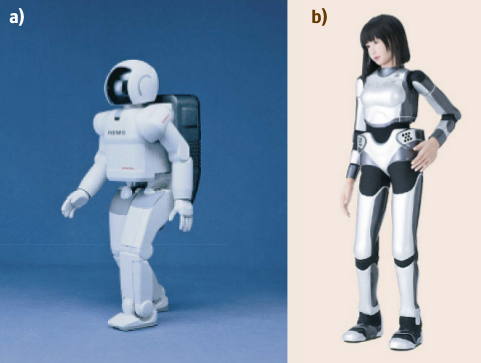
\includegraphics[scale=0.5]{images/asimov_and_HRP-4C.png}
	\caption{Ejemplos de robots humanoides (a) Asimov (2000); (b)HRP-4C (2009). Imagen tomada de: \cite{siciliano2016springer}.}		
\label{fig:humanoids}%(Ver página 423).
\end{figure}


			\subsubsection*{Análisis de estabilidad}

Para el control del sistema dinámico no lineal hay  un número de conceptos relativos para su seguridad y estabilidad:

\begin{itemize}
\item \textit{Puntos fijos} : Representan las posturas estáticas en cuáles el robot puede estar de pie de manera segura.

\item \textit{Ciclos límites}: Proveen una natural extensión del análisis de los puntos fijos para movimientos de caminata periódica.

\item \textit{Viabilidad}: La viabilidad es un concepto de invarianza controlada, que analiza el conjunto de estados del cual el robot es capaz de mantenerse de pie. Desafortunadamente esta propiedad puede ser intratable para el cómputo.

\item \textit{Controlabilidad}: La controlabilidad provee una ligera noción de restricción de viabilidad, analizando el conjunto de estados del cual el robot es capaz de retornar a un particular punto fijo.

\item \textit{Estabilidad robusta}: Examina las propiedades del sistema considerando el "peor de los casos" de las perturbaciones. Por instancias, un controlador robusto debería ser capaz de garantizar que un punto fijo es estable incluso si la estimación de masa del tronco tiene un error del $\pm$10\%.

\item \textit{Estabilidad estocástica}: El análisis estocástico provee herramientas para investigar la probabilidad de caer. Para muchos modelos de perturbaciones en robots el sistema caerá eventualmente (con probabilidad uno), pero el análisis puede revelar la distribución del tiempo de vida metaestable.

\item \textit{Estabilidad de entrada-salida}: En este análisis se trata una particular perturbación como una entrada, un criterio de rendimiento como salida e intenta calcular una ganancia relativa o sensibilidad del rendimiento del robot debido a esta entrada.

\item \textit{Márgenes de estabilidad}: El análisis de robustez puede ser difícil. En la práctica, los diseñadores del control a menudo se conforman con que el sistema se mantenga cómodamente lejos de los límites de estabilidad determinista.		

\end{itemize}

	\section{Aplicaciones en el juego de Futbol Soccer}	
		\subsubsection*{Futbol Soccer en el concurso RoboCup}
		La \textit{RoboCup Federation} es una iniciativa internacional para promover la inteligencia artificial y la tecnología robótica a través de la organización de competencias y encuentros científicos. Una de las categorías más famosas dentro de este concurso es el de fútbol soccer con robots humanoides (Humanoid League) cuyo objetivo es lograr que para la mitad del siglo XXI un equipo de robots humanoides autónomos sean capaces de ganar una partida de fútbol contra el recien campeón mundial de ese entonces, siguiendo las reglas oficiales de la FIFA.
		
		Las competencias de soccer comenzaron en el año de 1997 con simples y simulados robots con ruedas, desde entonces el desarrollo  fue creciendo hasta que en el 2002 se inauguró la liga de humanoides. Para ese entonces los principales retos eran comportamientos como caminar, patear y percibir objetos del ambiente, de esta manera, las mejoras en los mecanismos, la electrónica y control han hecho evolucionar el desarrollo para que la \textit{biomímesis} sea la más parecida a la de un humano.\citep{gerndt2015humanoid}
		
		\subsubsection*{Liga de robots humanoides de categoría \textit{TeenSize}}
		En los recientes años, la introducción de robots estandarizados, accesibles y de bajo costo ha tenido una formidable aceptación para el desarrollo e investigación de robots para soccer. Un ejemplo, es el humanoide \textit{DARwIn-OP} (Figura \ref{fig:Darwin_OP}), este robot cuenta con una plataforma estable, y algunos comportamientos de soccer están ya implementados, de modo que los nuevos desarrolladores tienen la oportunidad de enfocarse en tareas de más alto nivel para hacer los partidos más dinánmicos y complejos. \citep{schwarz2013humanoid}. 
		
		\textit{DARwIn-OP} (categorizado dentro de \textit{KidSize}) ha facilitado que los equipos lleguen a tener el número necesario de jugadores (robots) para los partidos, no obstante, para otras categorías en donde los robots tienden a tener mayor tamaño (\textit{TeenSize} o \textit{AdultSize}) no se llega a tener el número suficiente de jugadores para completar los equipos y algunos competidores se ven forzados a participar con robots hechos por ellos mismos. Consecuentemente esto altera el desempeño de los partidos y retraza el desarrollo de nuevos comportamientos. Para solucionar este problema fue desarrollado un primer prototipo de plataforma abierta basado el \textit{Darwin-OP} para la categoría \textit{TeenSize} llamado \textit{Nimbro-OP} (véase la sección 5.1) el cual tiene un diseño de fácil manufactura, ensamblaje y mantenimiento.	 

\begin{figure}
\centering
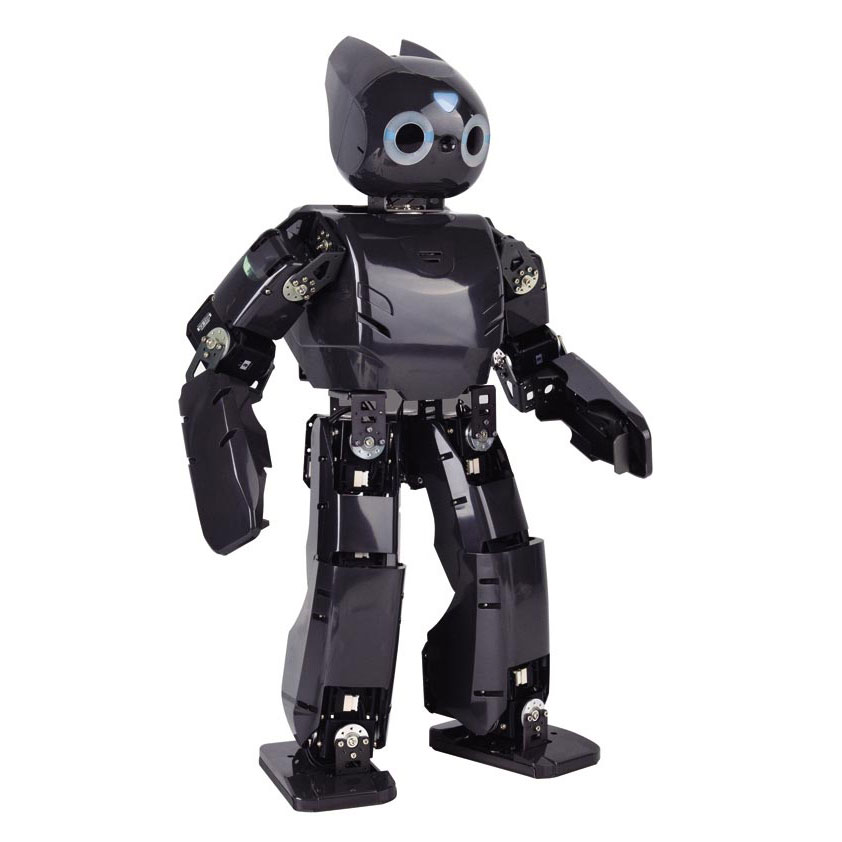
\includegraphics[scale=0.25]{images/Darwin_OP.jpg}
\caption{Robot Humanoide Darwin-OP (Imagen tomada de: http://openrobot.cl/es/robot-darwin-op/).}
\label{fig:Darwin_OP}
\end{figure}

	\section{Usos de la visión computacional}
	La \textit{visión computacional} es la transformación de información lumínica desde una imagen o video a hacia una \textit{nueva representación} de datos \cite{bradski2008learning}. Con esta nueva representación se pueden usar ciertas características de la luz capturada para transformarlas en variables numéricas que la computadora pueda abstraer y procesar (tómese de ejemplo la figura \ref{fig:camera_representation}).

\begin{figure}
\centering
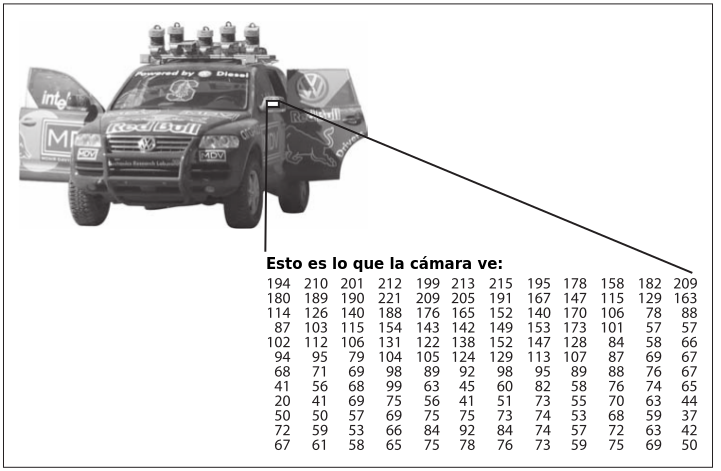
\includegraphics[scale=0.6]{images/new_representation_image.png}
\caption{Representación de cómo una imagen es representada por la computadora. Imagen modificada de: \cite{bradski2008learning}}
\label{fig:camera_representation}
\end{figure}

Para los fines de esta tesis, no es será necesario hacer uso de software para reconocimiento de formas o patrones, solamente se utilizarán funciones para segmentar objetos con base en su color, lo cual es muy conveniente para determinar la posición del objeto en el espacio. Tal y como se puede ver en el análisis matemático de la sección 4.1.
	
	\section{El Filtro de Kalman}
		\subsection*{Filtro de Kalman Discreto}
	En 1060 Rudolf Emil Kalman publicó su famoso \textit{paper} donde describe una forma sencilla para filtrar datos discretos de manera recursiva. Este método ha sido usado ampliamente en investigaciones y aplicaciones de ingeniería ya que resulta útil para la predicción de estados con base en modelos matemáticos y datos estadísticos. Por ejemplo, la posición y velocidad de un avión en vuelo, la temperatura de una caldera a la que se le está suministrando combustible o las lecturas dispersas de posición en un GPS.

	El Filtro de Kalman es un algoritmo computacionalmente eficiente cuyas ecuaciones matemáticas minimizan el error producido por el ruido inherente de las mediciones. Con la estimación es posible conocer con precisión el estado pasado, presente y futuro de un sistema, incluso si éste tiene un modelo de naturaleza desconocida.
	
		\subsection*{Proceso de estimación}
		El Filtro de Kalman aborda el problema de tratar de estimar el estado $x \in \Re^n$ de un proceso de tiempo discreto que es modelado con la ecuación diferencial \ref{eq:kalman_filter}.
		
\begin{equation}
\hat{x}_{n+1,n} = F \hat{x}_{n,n} + G \hat{u}_{n,n}
\label{eq:kalman_filter}
\end{equation}

	En donde $F$ es una matriz de nxn que relaciona el estado presente $n$ con el estado futuro $n+1$. $G$ es una matriz de nx1 que relaciona la entrada de control $u \in R^1$ al estado $x$. 
\\
	La medición $z \in \Re^m$, también conocida como vector de medición se puede modelar con la ecuación \ref{eq:measurement_equation}:

\begin{equation}
z_n = Hx_n+v_n
\label{eq:measurement_equation}
\end{equation}

En donde la matriz de observación $H$ de mxn es la que relaciona el estado $x_n$ con la medición $z_n$, el vector $v_n$ representa el ruido aleatorio en la medición. El Filtro de Kalman supone que el error en las mediciones debe tener una distribución normal, de esta manera la predicción de los estados tendrá un mayor grado de confiabilidad, por lo tanto la expresión \ref{eq:normal_distribution_R} representa cómo está distribuido el error del vector $v_n$. 

\begin{equation}
p(v) \sim N(0,R)
\label{eq:normal_distribution_R}
\end{equation}

Con el objetivo de encontrar una ecuación que calcule la estimación de un estado \textit{a posteriori} $\hat{x}_{n,n}$ como una combinación lineal de un estado \textit{a priori} $\hat{x}_{n, n-1}$ más una proporcional diferencia de la medición actual $z_n$ con la predicción $H\hat{x}_{n,n-1}$ se emplea la ecuación \ref{eq:posteriori_predicted}.

\begin{equation}
\hat{x}_{n,n} = \hat{x}_{n,n-1} + K_n (z_n-H\hat{x}_{n,n-1})
\label{eq:posteriori_predicted}
\end{equation}

$K_n$ es una matriz de nxm llamada \textit{Ganancia de Kalman}, esta ganancia está dada por la ecuación \ref{eq:k_gain} y su valor determina si es más confiable el valor de la medición o la predicción previa del modelo matemático.

\begin{equation}
K_n = P_{n,n-1}H^T(HP_{n,n-1}H^T+R_n)^{-1}
\label{eq:k_gain}
\end{equation}

Como puede observarse, cuando el error de covarianza de la medición $R_n$ se aproxima a cero, la ganancia $K_n$  tiene un mayor peso (cercano a uno). Por el contrario, cuando el error de covarianza \textit{a posteriori} $P_{n,n-1}$ se aproxima a cero, la ganancia $K_n$ obtiene menor peso (cercano a cero).
	La matriz de mxm $Q$ o \textit{matriz de error de proceso} describe el error causado por situaciones imprevistas, causados por ambientes irregulares o fallas mecánicas .	
\\
\\
	El algoritmo consta de dos fases, la fase \textit{predictiva} y la fase \textit{correctiva}. La fase predictiva consta de utilizar un modelo matemático para obtener las probables mediciones de un fenómeno. La fase correctiva obtiene los valores de la medición y las compara con las obtenidas con el modelo matemático, véase la figura \ref{fig:Kalman_scheme}.

\begin{figure}
\centering
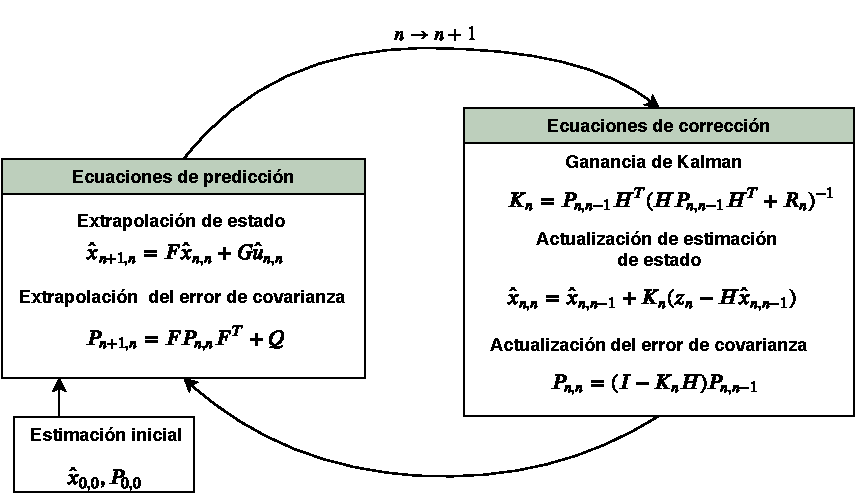
\includegraphics[scale=0.7]{images/kalman_algorithm.pdf}
\caption{Esquema ilustrativo del Filtro de Kalman. Diagrama Modificado de: \cite{welch1995introduction}}
\label{fig:Kalman_scheme}
\end{figure}

	Como ser vio, este filtro utiliza modelos matemáticos lineales, sin embargo en diversas situaciones, el modelo matemático no es lineal, y la predicción resulta ser errónea. Para solucionar esto, se puede implementar el Filtro de Kalman Extendido, que es básicamente el mismo tomando como lineal el modelo en ciertos intervalos de tiempo, y linealizando la predicción de la covarianza del proceso con base en la serie de Taylor. Véase la figura \ref{fig:extended_kalman_scheme}.

\begin{figure}
\centering
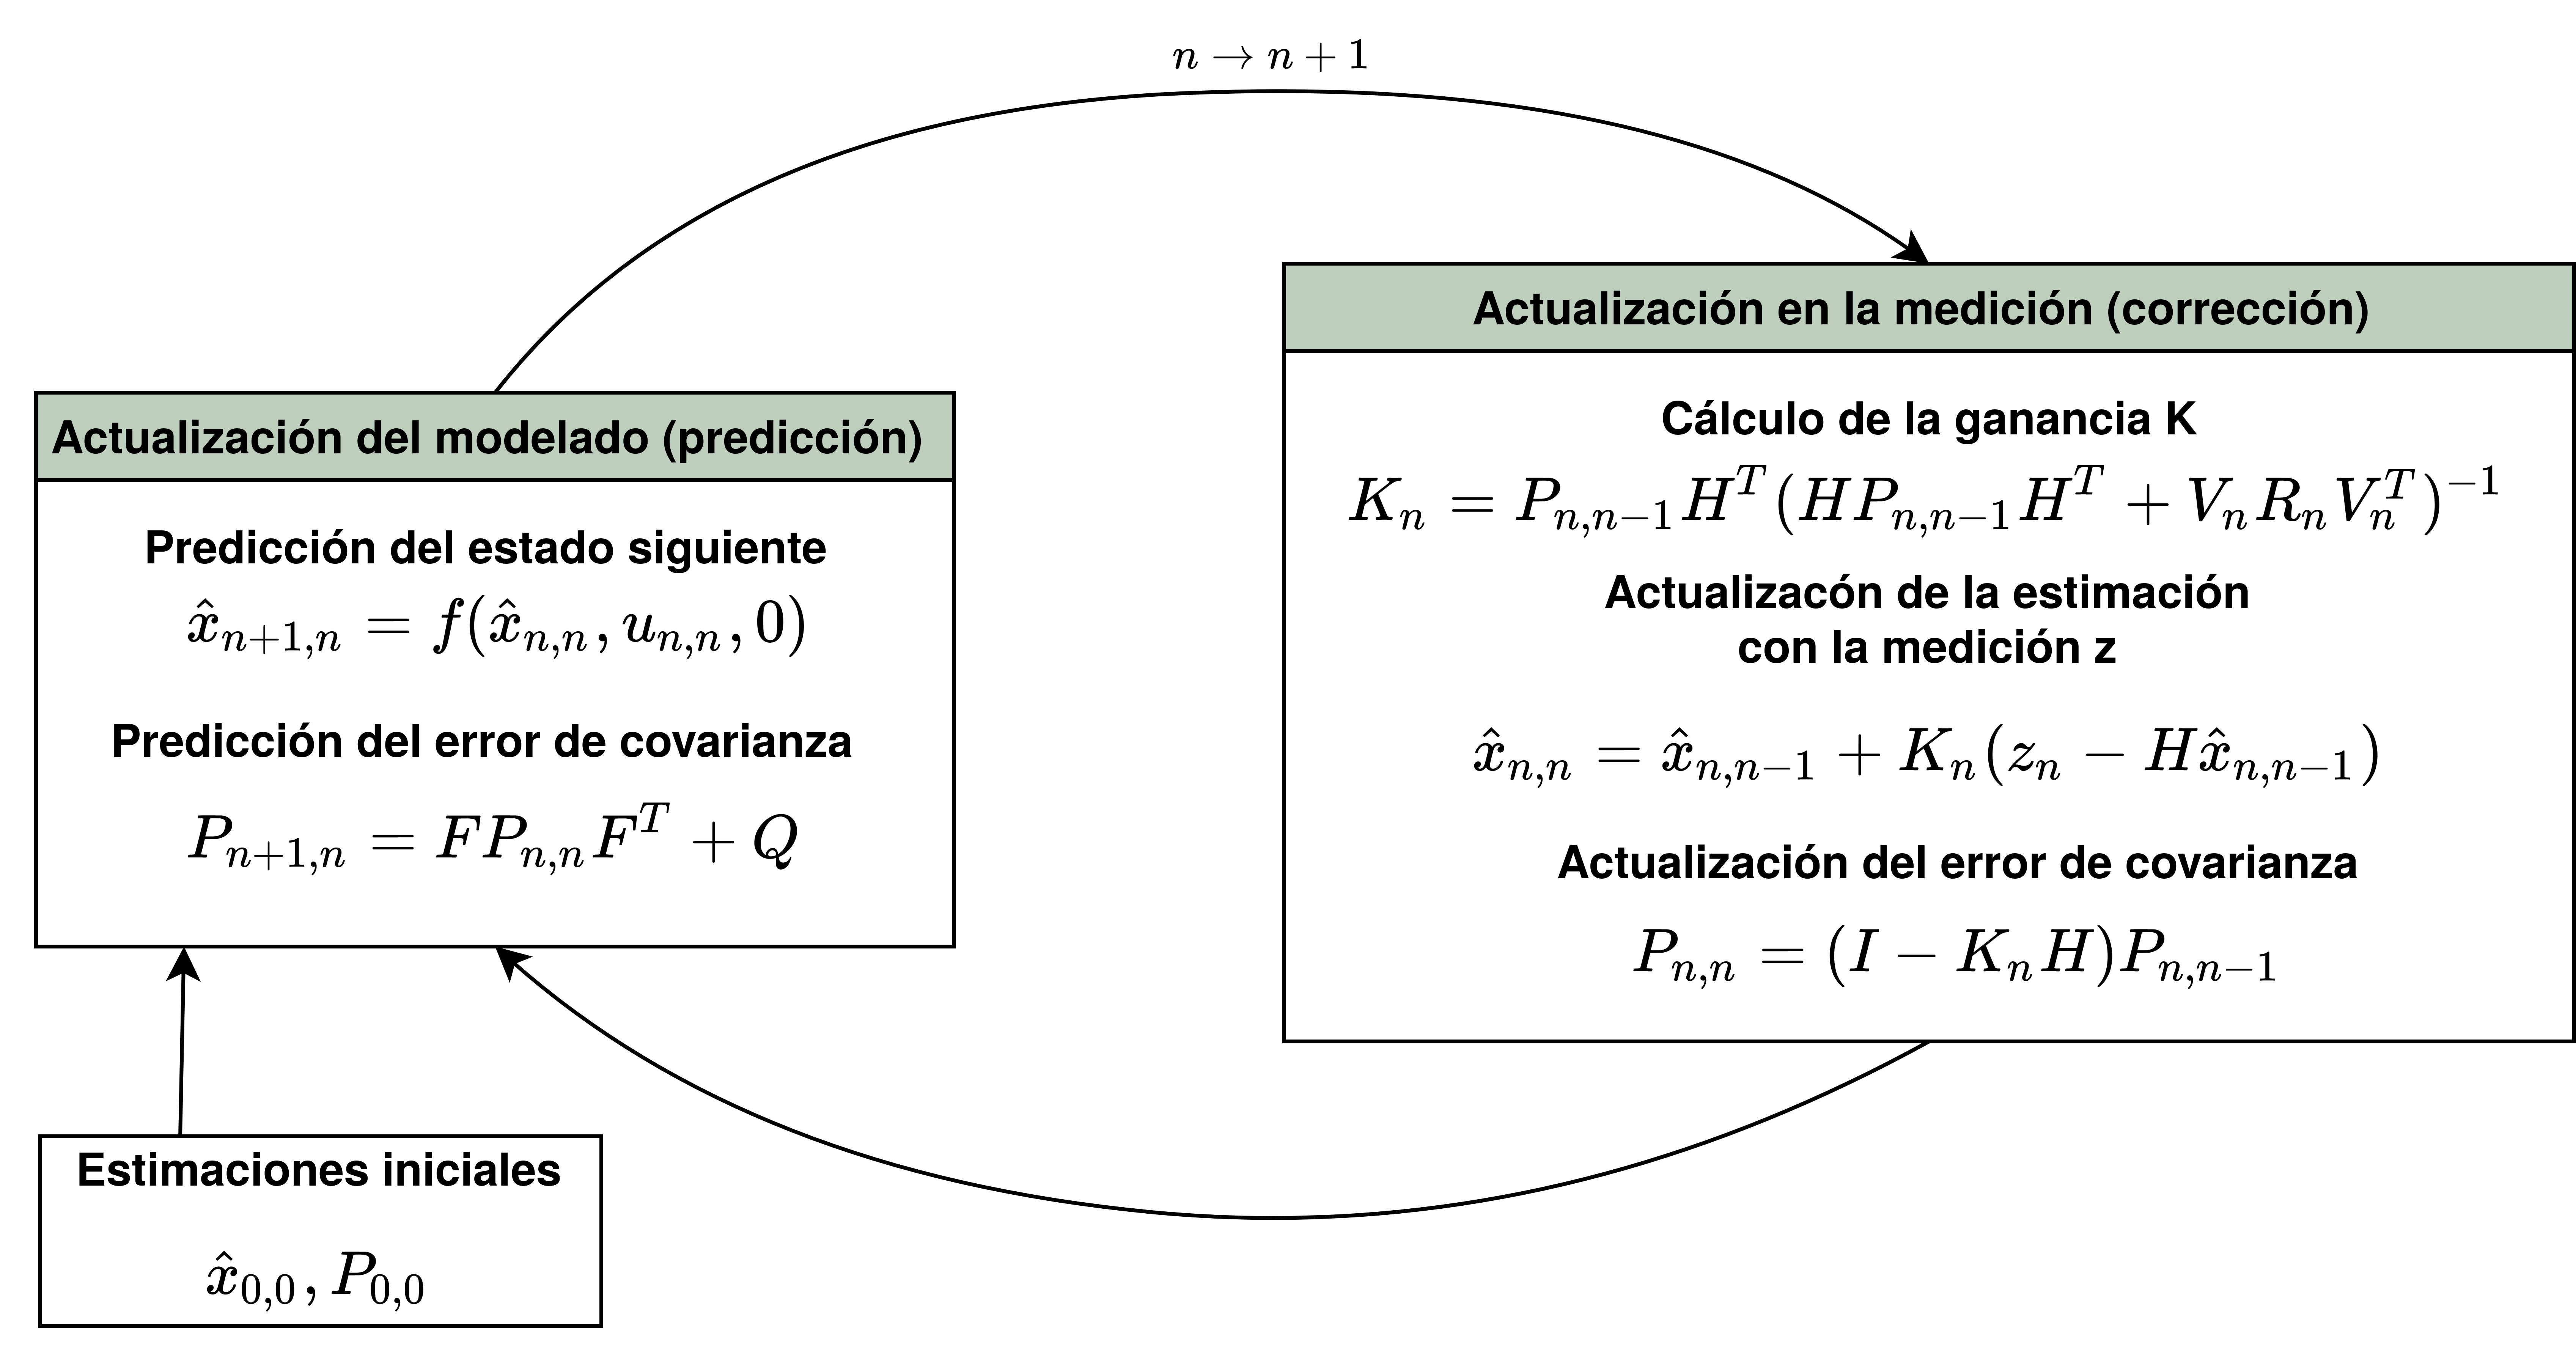
\includegraphics[scale=0.05]{images/extended_kalman_algorithm.png}
\caption{Esquema del Filtro de Kalman Extendido. Diagrama Modificado de: \cite{welch1995introduction}}
\label{fig:extended_kalman_scheme}
\end{figure}

En el capítulo 4 se deduce el modelo matemático del sistema de estimación, y se decide si se trabajará con el filtro extendido o el normal. 
	\section{Trabajo relacionado}
	
	Como ya se ha mencionado, la detección del balón es el principal objetivo para la categoría de \textit{Soccer Humanoids}. Esto representa un reto para los sistemas de visión computacional, el cual debe encargarse tanto de la detección como del cálculo de la posición con base en un sistema egocéntrico. Según los TDP \textit{(Team Description Paper)} se puede saber cómo los equipos han abordado este desafío en los recientes años, por lo que ayuda en gran medida para saber qué técnicas se pueden reimplementar o mejorar según la necesidad. 
\\	

	En los siguientes párrafos se resumen los métodos utilizados por los equipos de distintos países, así será fácil diferenciar con los métodos implementados de esta tesis.
	
	\subsection*{ITAndroids}
	El equipo \textit{ITAndroids} del Instituto Tecnológico de Aereonáutica de Brasil implementó un sistema basado en los sistemas de visión de los humanoides de la plataforma estándar. Tomaron como punto de partida la segmentación por color con algoritmos hechos en MATLAB y funciones de OpenCV como \textit{Hough Circle Transform} para la detección correcta del objetivo, tal y como se ve en la Figura \ref{fig:ITAndroids_vision}.
	
\begin{figure}
\centering
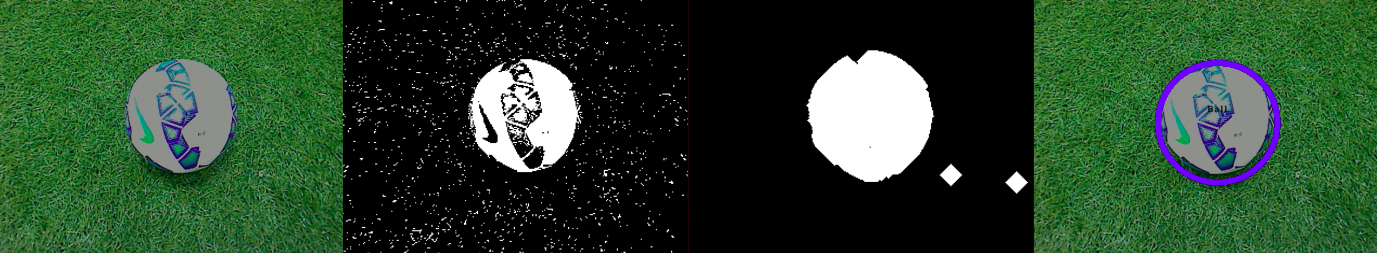
\includegraphics[scale=0.25]{images/ITAndroids_vision.png}
\caption{Proceso de vision implementado por ITAndroids. Imagen tomada de: \cite{davi2017ITAndroids}}
\label{fig:ITAndroids_vision}
\end{figure}

	Debido al ruido inherente en el procesamiento de imágenes, un Filtro de Kalman es empleado para estimar la posición más probable si es que un objeto del mismo color del balón es detectado.
	
	Ya que se hace el reconocimiento del balón, se procede a calcular su posición relativa respecto al humanoide, transformando las coordenadas bidimensionales obtenidas por la imagen a tridimensionales haciendo uso de un método similar al de esta tesis (véase la Sección 4), suponiendo que la posición del balón en la coordenada \textit{z} es siempre 0 y calculando la cinemática directa desde la posición de la cámara a la posición de dicho objetivo.
	
	 \subsection*{NimbRo TeenSize}
	 Debido a las nuevas reglas dadas por el comité organizador de la RoboCup en cuanto al color del balón (blanco como en las competencias de la FIFA), el equipo \textit{NimbRo} de la Universidad de \textit{Friedrich-Wilhelms} de Alemania optó por utilizar un sistema de reconocimiento que no se base sólo en color, pues las líneas divisorias de las canchas o la portería tienen la misma tonalidad. Es por eso que su sistema de reconocimiento está basado en histogramas HOG (histogram of oriented gradients).
	
	 Con el reconocimiento debidamente implementado, se usan las Transformaciones Homogéneas para obtener la posición del balón con cinemática directa, de este modo resulta muy útil la biblioteca \textit{tf2} de ROS. No obstante, aunque las posiciones del robot están bien definidas, algunas variaciones del hardware pueden dar pauta al error en la medición. Para resolver estos fallos este equipo usó el método de Nelder-Mead que consiste en hacer una triangulación convergente para las probables posiciones del balón.
	 
	 \subsection*{T-Flow}
	 Otra forma para realizar la detección de objetos es obteniendo una forma tridimensional específica con una cámara estéreo, tal y como lo hizo el equipo \textit{T-Flow} del \textit{Centro de Investigación de Robótica} del Politécnico de Indonesia. 
	 

	 Este equipo emplea una cámara estéreo para obtener un par de imágenes, remapear y formar una imagen tridimensional con profundidad aproximada, para posteriormente compararse con un patrón esférico como lo es el balón. 	 


	 El sistema de estereo-visión resulta ser muy útil y sencillo para la detección y posicionamiento del objeto, no obstante, se requiere un elevado coste computacional.
	 
	\subsection*{Ichiro}
	De una manera muy similar al robot del Laboratorio de Bio-robótica de la UNAM, los humanoides del equipo \textit{Ichiro} del \textit{Instituto Tecnológico Diez de Noviembre} de Indonesia, poseen una web-cam Logitech C922 con alta definición.
	
	En la detección del balón este equipo emplea un método de Patrones de Binarios Locales el cual es un descriptor de texturas que toma como base la transformación de las imágenes a escala de grises, para posteriormente tomar como contorno los cambios de tonalidad, este método representa bajo costo computacional y hace la segmentación más independiente a los cambios de luz. 
\\

	Como se observó en estos párrafos, existen distintos procedimientos para la detección y localización tridimesional del objeto, las cuales resultan muy prometedoras. No obstante, poco se menciona sobre la detección de objetos en movimiento, y los filtros empleado sólo comprenden modelos estáticos, por lo que esta tesis busca ampliar las fronteras de los algoritmos comunmente empleados. 	 